%KECReportFormat.tex
%%%%%%%%%%%%%%%%%%%%%%%%%%%%%%%%%%%%%%%%%%%%%%%%%%%%%%%%%%%%%%%%%%%%%%%%%%%
%DO NOT MAKE CHANGES IN THIS FILE

\documentclass[12pt, a4paper]{report}
\usepackage[left = 1.5in, right = 1in, top = 1in, bottom = 1in]{geometry}%for margin
\usepackage{amsfonts, amsmath, amssymb} %for mathematical equations
\usepackage{graphicx} %for images
\usepackage{times} %font Times New Roman Font
\usepackage{float} %required if you use H(strictly here) position for floats
\usepackage[skip = 8pt,tableposition=top, figureposition=bottom]{caption}%adjust spacing of captions and specify where captions are
\usepackage{hyperref} % for easy Navigation in document, also puts links in TOC, LOF, LOT...
\usepackage{setspace} %to change line spacing in some portion \singlespacing \onehalfspacing \doublespacing
\usepackage{acro} %for List of Abbrreviation and Symbol
\acsetup{first-style = short} % set to display only short form on the command \ac{}

%packages required for complex tables
\usepackage{bigstrut} 
\usepackage{multirow}

\renewcommand{\contentsname}{Table of Contents} %Change TOC Heading ... default is "Contents" 

\parindent 0pt	%removes the indent in paragraph
\setlength{\parskip}{18pt}	%for paragraph spacing
\renewcommand{\baselinestretch}{1.5}   %Line Spacing = 1.5 line-spaces

%to reduce spacing in sections
\usepackage{titlesec}
\titlespacing*{\section}{0pt}{0pt}{0pt} %left, top, bottom spacings
\titlespacing*{\subsection}{0pt}{0pt}{0pt}
\titlespacing*{\subsubsection}{0pt}{0pt}{0pt}
\titlespacing*{\paragraph}{0pt}{0pt}{0pt}
\titlespacing*{\subparagraph}{0pt}{0pt}{0pt}

%adjust fontsizes\ of sections
\titleformat*{\section}{\fontsize{14pt}{18pt}\bfseries}
\titleformat*{\subsection}{\fontsize{13pt}{18pt}\bfseries}
\titleformat*{\subsubsection}{\fontsize{12pt}{18pt}\bfseries}
\titleformat*{\paragraph}{\fontsize{12pt}{18pt}\bfseries}
\titleformat*{\subparagraph}{\fontsize{12pt}{18pt}\bfseries}

%to reduce separation between points in list
\usepackage{enumitem}
\setlist[enumerate]{nosep} % no separation between items in enumerate
\setlist[itemize]{nosep} % no separation between items in itemize
%use \vspace{-18pt} before list to reduce paragraph spacing between list and preceeding paragraph.

%Changes for Chapter Heading Spacing and formats for numbered chapters
\makeatletter
\def\@makechapterhead#1{%
  %\vspace*{50pt}%
  {  \MakeUppercase{\ifnum \c@secnumdepth >\m@ne
        \fontsize{16pt}{1}\bfseries \@chapapp \space \thechapter\vspace{5pt}\\
    \fi
    \interlinepenalty\@M
     \bfseries #1}\par\nobreak
    %\vskip 0pt
  }}
\makeatother

%%%%%%%%%%%%%%%%%%%%%%%%%%%%%%%%%%%%%%%%%%%%%%%%%%%%%%%%%%%
%to adjust Heading spacings and fonts For unnumbered chapters, TOC, LOF ...
\makeatletter
% Redefine the \chapter* header macro to remove vertical space
\def\@makeschapterhead#1{%
  %\vspace*{50\p@}% Remove the vertical space
  {\newpage \parindent \z@ \raggedright
    \normalfont
    \interlinepenalty\@M
    \center \fontsize{16pt}{1} \bfseries \MakeUppercase{#1}\par\nobreak
    %\vskip 18\p@ % adjust space after heading 18pt
  }}
\makeatother 
%%%%%%%%%%%%%%%%%%%%%%%%%%%%%%%%%%%%%%%%%%%%%%%%%%%%%%%%%%%

%%%%%%%%%%%%%%%%%%%%%%%%%%%%%%%%%%%%%%%%%%%%%%%%%%%%%%%%%%%%%%%%%%%%%%%%%%%
% newcommand for generating Cover Page
\newcommand{\KECcoverpage}
{
\begin{titlepage}
\begin{center}
\Large{\textbf{KANTIPUR ENGINEERING COLLEGE}}\\
\large{\textbf{(Affiliated to Tribhuvan University)}}\\
\large{\textbf{Dhapakhel, Lalitpur}}\\
\vfill	%vertically fill the space 
\begin{figure}[h] % h: put logo "here"
\begin{center}

\includegraphics[width=25mm, height = 25mm]{images/logo.png}
\end{center}
\end{figure}

\large{\textbf{[Subject Code: \subCode]}}\\ %Change This Line
\large{\textbf{A \MakeUppercase{\project} \MakeUppercase{\doc} ON}}\\ %Change This Line
\Large{\textbf{\MakeUppercase{\projectTitle}}}\\

\vfill	%vertically fill the space 
\large{\textbf{Submitted by:}}\\
\large{\textbf{\submittedBy}}\\
\vfill	%vertically fill the space 
\textbf{A \MakeUppercase{\project} SUBMITTED IN PARTIAL FULFILLMENT OF THE REQUIREMENT FOR THE DEGREE OF \MakeUppercase{\degree}}\\

\vfill	%vertically fill the space 
\large{\textbf{Submitted to:}}\\
\large{\textbf{\submittedTo}}\\
\vfill
\large{\textbf{\defMonth, \defYear}}
\pagebreak
\end{center}
\end{titlepage}
}
%%%%%%%%%%%%%%%%%%%%%%%%%%%%%%%%%%%%%%%%%%%%%%%%%%%%%%%%%%%%%%%%%%%%%%%
% newcommand for generating Cover Page
%Title Page
\newcommand{\KECtitlepage}
{
\begin{titlepage}
\begin{center}
\Large{\textbf{\MakeUppercase{\projectTitle}}}\\

\vfill	%vertically fill the space 

\large{\textbf{Submitted by:}}\\
\large{\textbf{\submittedBy}}\\


\ifhassupervisor % Displays Supervisor name only if \hassupervisortrue
	\vfill	%vertically fill the space 
	\large{\textbf{Supervised by:}}\\
	\large{\textbf{\supervisor}}\\
	\large{\textbf{\degSup}}\\
\fi

\vfill	%vertically fill the space 
\textbf{A \MakeUppercase{\project} SUBMITTED IN PARTIAL FULFILLMENT OF THE REQUIREMENT FOR THE DEGREE OF \MakeUppercase{\degree}}\\

\vfill	%vertically fill the space 
\large{\textbf{Submitted to:}}\\
\large{\textbf{\submittedTo}}\\
\large{\textbf{Kantipur Engineering College}}\\
\large{\textbf{Dhapakhel, Lalitpur}}\\

\vfill
\large{\textbf{\defMonth, \defYear}}
\thispagestyle{empty}\\ %to remove page number
\pagebreak
\end{center}
\end{titlepage}
}
%%%%%%%%%%%%%%%%%%%%%%%%%%%%%%%%%%%%%%%%%%%%%%%%%%%%%%%%%%%%%%%%%%%%%%
%command for copyright page
\newcommand{\KECcopyright}
{
\chapter*{Copyright}%Required only for Final Defense of Major Project
\addcontentsline{toc}{chapter}{Copyright}
The author has agreed that the library, Kantipur Engineering Collage, may make this report freely available for inspection. Moreover the author has agreed that permission for extensive copying of this report for scholarly purpose may be granted by the supervisor(s), who supervised the project work recorded herein or, in their absence, by the Head of the Department wherein this project was done. It is understood that due recognition will be given to the author of this report and to the \submittedTo, Kantipur Engineering College in any use of the material of this report. Copying or publication or other use of this report for financial gain without approval of the \submittedTo, Kantipur Engineering College and author’s written permission is prohibited.\par Request for permission to copy or to make any other use of the material in this report in whole or in part should be addressed to:

Head\\
\submittedTo\\
Kantipur Engineering College\\
Dhapakhel, Lalitpur\\
Nepal
}
%%%%%%%%%%%%%%%%%%%%%%%%%%%%%%%%%%%%%%%%%%%%%%%%%%%%%%%%%%%%%%%%%%%%%%
%command for Approval Letter
\newcommand{\KECapproval}
{
\chapter*{Kantipur Engineering College
\vskip -10pt}%Required only for Final Defense of Major Project
\begin{center}
\fontsize{12.8pt}{1} %size decreaced to adjust department name in single line
\textbf{
\MakeUppercase{\submittedTo}\\ %for department name
}
\vskip 10pt
\fontsize{16pt}{1}
\textbf{APPROVAL LETTER}
\end{center}
\vskip -16pt
\addcontentsline{toc}{chapter}{Approval Letter}%
The undersigned certify that they have read and recommended to the Institute of Engineering for acceptance, a project report entitled "\projectTitle " submitted by \\
\submittedBy \\
in partial fulfillment for the degree of \degree. \par
{\vspace{25pt}
..........................................\\
Supervisor\\
\supervisor \\
\degSup\\
\vspace{25pt}\\
..........................................\\
External Examiner\\
\external\\
\degExternal\\
\vspace{25pt}\\
..........................................\\
\hod\\
Head of Department\\
\submittedTo
\vspace{10pt}\\
Date: \defMonth\space\defDay ,\space \defYear
\singlespacing\par
} %single spacing for the texts inside {}
}

%command for list of abbreviations
\newcommand{\KECloa}
{
\chapter*{List of Abbreviations}
\addcontentsline{toc}{chapter}{List of Abbreviations}
\vskip -42pt % to reduce space due to invisivle acronym class name
{
\singlespacing
\printacronyms[include-classes=abbr, name= ]
}

}

%command for list of symbols
\newcommand{\KEClos}
{
\chapter*{List of Symbols}
\addcontentsline{toc}{chapter}{List of Symbols}
\vskip -42pt % to reduce space due to invisivle acronym class name{
{
\singlespacing
\printacronyms[include-classes=symbol, name= ]
}
}

%command to adjust toc, lof, lot spacing
\newcommand{\KECadjusttocspacings}
{
\parskip 0pt % to remove paragraph spacing in TOC, LOF ...
\renewcommand{\baselinestretch}{0.1} % to adjust line spacing in toc
\newcommand*{\noaddvspace}{\renewcommand*{\addvspace}[1]{}}
\addtocontents{lof}{\protect\noaddvspace} %remove extra vertical space in LOF
\addtocontents{lot}{\protect\noaddvspace} %remove extra vertical space in LOT
} %includes the file KecReportFormat.tex that include all necessary formattings
%%%%%%%%%%%%%%%%%%%%%%%%%%%%%%%%%%%%%%%%%%%%%%%%%%%%%%%%%%%%%%%%%%%%%%%%%%%
%Define Macros for Details of your Project
\newcommand{\project}{Major Project} %Specify "Major Project" or "Minor Project"
\newcommand{\projectTitle}{Network Intrusion Detection System Using LSTM} %specify "Title" of Your Project
\newcommand{\doc}{Final Report} % specify the document you are preparing eg. "Proposal", "Mid-Term Report" or "Final Report" 
% Note that You have to sibmit "Final Report" for Pre-final defense as well.
\newcommand{\subCode}{CT755} %specify Subject of Your Project
\newcommand{\degree}{Bachelor in Computer Engineering} %specify your degree
\newcommand{\submittedBy}%Specify Names and Roll/Symbol Numbers of the Project Group Members
{
%Edit Member Names and Roll/Symbol No. and adjust width (\makebox[width]) if necessary 
\makebox[7cm]{Aman Devkota  \hfill[KAN076BCT010]}\\
\makebox[7cm]{Ankur Karmacharya  \hfill[KAN076BCT013]}\\
\makebox[7cm]{Prashad Adhikary  \hfill[KAN076BCT056]}
%\makebox[9cm]{Member Name \hfill [Roll/Symbol No.]}\\
} % Note that You must write your "Symbol Numbers"(Exam Roll Numbers) for Final Defenses

\newcommand{\submittedTo}{Department of Computer and Electronics Engineering} %specify your department
\newcommand{\hod}{Er. Rabindra Khati} %specify Head ot the department
\newcommand{\defYear}{2024} %Defense Year
\newcommand{\defMonth}{February} %Defense Month- January, February, ...
\newcommand{\defDay}{25} %specify Defense Day- 1, 2, ...

\newif\ifhassupervisor
\hassupervisortrue % to display supervisor name use command- \hassupervisortrue
\newcommand{\supervisor}{Babu Ram Dawadi} % Specify Name of Supervisor for Major Project (write "none" if no Supervisor is assigned)
\newcommand{\degSup}{Supervisor's Designation\\Second Line of Designation (if required)} %Specify Designation of Supervisor for Major Project, use multiple lines (\\) if necessary
\newcommand{\external}{External's Name} %Specify Name of External for Major Project (Required for Black Book)
\newcommand{\degExternal}{External's Designation\\Second Line of Designation (if required)} %Specify Name of External for Major Project (Required for Black Book) , use multiple lines (\\) if necessary
%%%%%%%%%%%%%%%%%%%%%%%%%%%%%%%%%%%%%%%%%%%%%%%%%%%%%%%%%%%%%%%%%%%%%%%%%%%

%%%%%%%%%%%%%%%%%%%%%%%%%%%%%%%%%%%%%%%%%%%%%%%%%%%%%%%%%%%%%%%%%%%%%%%%%%%

%%%%%%%%%%%%%%%%%%%%%%%%%%%%%%%%%%%%%%%%%%%%%%%%%%%%%%%%%%%%%%%%%%%%%%%%%%%%%%%%%%%%%%%%%%%%%%%%%%%%

%%%%%%%%%%%%%%%%%%%%%%%%%%%%%%%%%%%%%%%%%%%%%%%%%%%%%%%%%%%%%%%%%%%%%%%%%%
%The Document
\setcounter{tocdepth}{3}
\setcounter{secnumdepth}{3}
\begin{document}

\KECcoverpage  
\KECtitlepage
\pagenumbering{roman} % starts pagenumberins in Roman numerals i, ii, ...

%Copyright Page is required for FINAL REPORT only. Comment this section for other Reports.
%\KECcopyright % defined in KECReportFormat.tex

%Approval Page is required for FINAL(Black Book Binded) REPORT of MAJOR PROJECT only. Comment this section for other Reports. 
%\KECapproval % defined in KECReportFormat.tex

\chapter*{Abstract} % The summary of your report
\addcontentsline{toc}{chapter}{Abstract}%to include %this chapter in TOC 
blablablaa
\par
\textbf{\textit{Keywords$-$}} \emph{LSTM, SDN,  ,}

\chapter*{Acknowledgment}
\addcontentsline{toc}{chapter}{Acknowledgment}%to include this chapter in TOC
We would like to express sincere gratitude to Department head Er. Rabindra Khati, Project Co-ordinator Er. Bishal Thapa and all the faculty members of Kantipur Engineering College for the continuous support during this project for their patience, motivation,enthusiasm, and immense knowledge. Their guidance helped us in all time of research, development and implementation of this project.\par
Finally we would like to thank our family and friends for all the support and encouragement.\par
%to display members name under Acknowledgement
\begin{flushright}
\vskip -20pt
\setstretch{1.2}
\submittedBy

\end{flushright}

%to adjust spacings for TOC, LOF, LOT
{
%%%%%%%%%%%%%%%%%%%%%%%%%%%%%%%%%%%%%%%%%%%%%%%%%%%%%%%%%%%%%%%%%%%%%%%%%%%
%TOC, LOF and LOT
\KECadjusttocspacings % defined in KECReportFormat.tex to adjust spacings
\makeatletter
% to add vskip of 18 point which is reduced when parskip is set to 0 in \LECadjustspacings
\def\@makeschapterhead#1{%
  %\vspace*{50\p@}% Remove the vertical space
  {\newpage \parindent \z@ \raggedright
    \normalfont
    \interlinepenalty\@M
    \center \fontsize{16pt}{1} \bfseries \MakeUppercase{#1}\par\nobreak
   % \vskip 18\p@ % adjust space after heading 18pt
  }}
\makeatother 

\tableofcontents % prints table of contents
\listoffigures % prints list of figures
\addcontentsline{toc}{chapter}{List of Figures}
%\listoftables % prints list of table
%\addcontentsline{toc}{chapter}{List of Tables}
}
%%%%%%%%%%%%%%%%%%%%%%%%%%%%%%%%%%%%%%%%%%%%%%%%%%%%%%%%%%%%%%%%%%%%%%%%%%%
\chapter*{List of Abbreviations}
\textbf{DOS}: Denial of Service\\
\textbf{FN}: False  Negative \\
\textbf{FP}: False Positive\\
\textbf{IDS}: Intrusion Detection System\\
\textbf{LSTM}: Long Short Term Memory\\
\textbf{R2L}: Root to Local \\
\textbf{TN}: True Negative\\
\textbf{TP}: True Positive\\
\textbf{U2R}: User to Root\\
\addcontentsline{toc}{chapter}{List of Abbreviations}
%comment this chapter if you don't have List of Abbreviations
%\KECloa % defined in KECReportFormat

%comment this chapter if you don't have List of Symbols
%\KEClos % defined in KECReportFormat

\newpage
\pagenumbering{arabic} % starts pagenumbering in arabic numerals

\chapter{Introduction}
\vspace{-18pt}
\section{Background}\label{sec:bkgrnd}%label your section if you require to refer them somewhere else in your document.
\vspace{-18pt}
%nw3
With the increasingly deep integration of the Internet and society, the Internet is changing the way in which people live, study and work, but the various security threats that we face are becoming more and more serious. How to identify various network attacks, especially unforeseen attacks, is an unavoidable key technical issue. An Intrusion Detection System (IDS), a significant research achievement in the information security field, can identify an invasion, which could be an ongoing invasion or an intrusion that has already occurred. In fact, intrusion detection is usually equivalent to a classification problem, such as a binary or a multi class classification problem, i.e., identifying whether network traffic behavior is normal or anomalous, or a five-category classification problem, i.e., identifying whether it is normal or any one of the other four attack types: Denial of Service (DOS), User to Root (U2R), Probe (Probing) and Root to Local (R2L). In short, the main motivation of intrusion detection is to improve the accuracy of classifiers in effectively identifying the intrusive behavior.\par
Machine learning methodologies have been widely used in identifying various types of attacks, and a machine learning approach can help the network administrator take the corresponding measures for preventing intrusions. However, most of the traditional machine learning methodologies belong to shallow learning and often emphasize feature engineering and selection; they cannot effectively solve the massive intrusion data classification problem that arises in the face of a real network application environment. With the dynamic growth of data sets, multiple classification tasks will lead to decreased accuracy. In addition, shallow learning is unsuited to intelligent analysis and the forecasting requirements of high-dimensional learning with massive data. In contrast, deep learners have the potential to extract better representations from the data to create much better models. As a result, intrusion detection technology has experienced rapid development after falling into a relatively slow period.\cite{yin2017deep}%chinese
\par
A well-known method of securing the network is through implementing an Intrusion Detection System (IDS). IDS was originally implemented in 1980. The main aim of their work was to introduce a mechanism which differentiates between benign activities from malicious ones. Further research was carried out to optimizing this methodology to aid monitoring the network traffic in case of attacks, this system is now known as Network Intrusion Detection System (NIDS) . In NIDS, the detection system is inspecting the incoming and outgoing network traffic from all hosts in real time and based on certain criteria, it can detect and identify the attack, then, take the suitable security measures to stop or block it, which significantly reduces the risk of damage to the network. However, due to the rapid increase in the complexity of the cyber-security attacks, the current methods used in NIDS are failing to sufficiently address this issue.\cite{al2020using}
\par 
IDSs can be divided into two categories according to the main detection technology: misuse detection and anomaly detection. Misuse detection is a knowledge-based detection technology. A misuse detection system needs to clearly define the features of the intrusion, then identify the intrusion by matching the rules. Misuse detection can achieve a high accuracy and low false alarm rate. However, it needs to build a feature library and cannot detect unknown attacks. In contrast, anomaly detection is a behavior-based detection technology. First, it needs to define the normal activities of a network, and then check whether the actual behavior has deviated from the normal activities. Anomaly detection needs only to define a normal state of a specific network, without prior knowledge of intrusion. Thus, it can detect unknown attacks, although there may be a high false alarm rate. At present, network structure is becoming more and more complicated, and intrusion methods are following the trend of diversification and complication, creating more challenges for IDSs.\par 
The recurrent neural network (RNN) has failed to become a mainstream network model in the past few years due to difficulties in training and computational complexity. In recent years, with the development of deep learning theory, RNN began to enter a rapid development period. Currently, RNN has already been applied successfully to handwriting and speech recognition. The main feature of RNN is that it circulates information in a hidden layer which can remember information processed previously, leading to a structural advantage for the processing of time series information. Correspondingly, many intrusion behaviors can be abstracted as specific time series of events from the underlying network. So, RNN is considered suitable for building an IDS.\cite{xu2018intrusion}
\par 
\section{Problem Statement}
\vspace{-18pt}
The existing Network Intrusion Detection Systems face challenges in accurately and efficiently detecting and preventing network intrusions, thereby compromising the overall security of computer networks. These challenges include high false-positive rates, limited scalability, inability to detect novel or sophisticated attacks, and the difficulty in distinguishing between legitimate and malicious network traffic. Addressing these issues is crucial to enhance the performance and reliability of NIDS, enabling proactive identification and prevention of network intrusions while minimizing false alarms.
\section{Objectives}
\vspace{-18pt}
The primary objective of this project:
\vspace{-18pt}
\begin{enumerate}[label=\roman*.]
\item To develop a robust and accurate system that can effectively detect and notify network intrusions or malicious activities within a computer network.
\end{enumerate}
\section{Project Features}
\vspace{-18pt}
The project will be able to accomplish following:
\vspace{-18pt}
\begin{itemize}
\item Anomaly Detection
\item Real-time Monitoring
\item Traffic Preprocessing
\end{itemize}
\section{Application Scope}
\vspace{-18pt}
Network Intrusion Detection System has various applications in areas such as Enterprise networks, Internet Service Providers(ISPs), Cloud Computing environment, Government networks and so on. The application scope of network intrusion detection systems using deep neural networks extends beyond these areas, as network security is crucial in nearly every sector that relies on secure and reliable communication. By deploying these systems, organizations can proactively detect and respond to network intrusions, minimize the impact of attacks, and protect their assets, data, and operations from potential threats.
\section{System Requirement}
\vspace{-18pt}
\subsection{Development Requirements}
\vspace{-18pt}
\subsubsection{Software Requirements}
\vspace{-10pt}
\begin{itemize} 
\item Windows/Linux/Mac
\item VMware/Virtualbox
\item Mininet, POX controller
\item Jupyter Notebook
\item Python IDE
\end{itemize}
\subsubsection{Hardware Requirements}
\vspace{-10pt}
\begin{itemize}
\item PC with at least 4-8 GB RAM
\item  Higher graphics of at least 2 GB
\end{itemize}
\subsection{Deployment Requirements}
\vspace{-18pt}
\subsubsection{Software Requirements}
\vspace{-10pt}
\begin{itemize}
\item Windows/Linux/Mac
\item VMware/Virtualbox
\item Mininet, POX controller
\end{itemize}
\vspace{-10pt}
\subsubsection{Hardware Requirements}
\vspace{-10pt}
\begin{itemize}
\item More than 1.5 GHz clock speed
\item Minimum 4 GB RAM
\end{itemize}
\label{tblSampleTable}
%\end{table}
\section{Project Feasibility}
\vspace{-18pt}
\subsection{Technical Feasibility}
\vspace{-18pt}
The technical feasibility assessment is focused on gaining in understanding of the present technical resources required by the system and their applicability to the expected needs of the proposed system. Regarding the proposed system, the technical requirement includes a PC.
\vspace{-18pt}
\subsection{Operational Feasibility}
\vspace{-18pt}
The user will not need any formal knowledge about programming so our project is operationally feasible.
\vspace{-18pt}
\subsection{Economic Feasibility}
\vspace{-18pt}
The purpose of the economic feasibility assessment is to determine the positive economic benefits to the user that the proposed system will provide. Most of the software used for the development is free. Thus, the project is economically feasible.
\vspace{-18pt}
\subsection{Schedule Feasibility}
\begin{figure}[!h] % tbh means top, bottom or here (priority: left to right)
\begin{center}
	%
\includegraphics[width = 3in]{images/logo.png}
	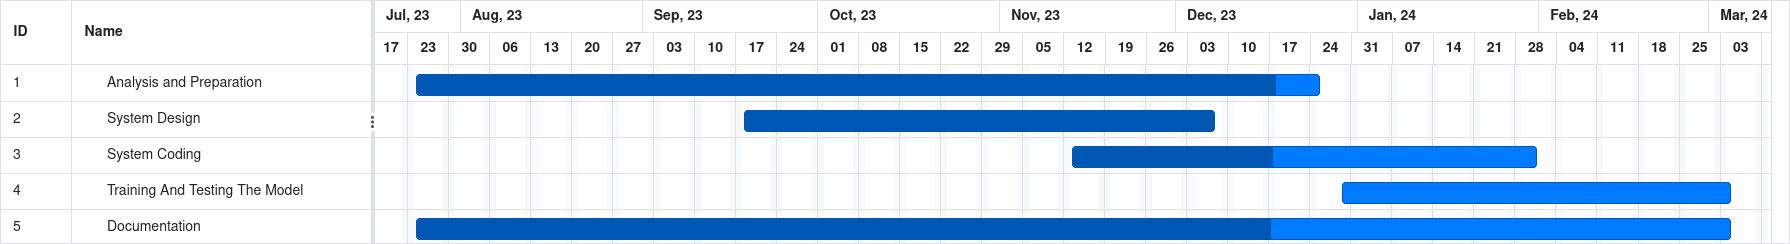
\includegraphics[width=6in,height=2in
	]{images/real_n.png} 
	\caption{Gantt Chart} %figure name
	\label{figGanttChart} % for referencing
\end{center}
\end{figure}
\chapter{Literature Review}
\vspace{-18pt}
\section{Related Projects}
\vspace{-18pt}
\subsection{Suricata}
\vspace{-18pt}
Suricata is a high performance, open source network analysis and threat detection software used by most private and public organizations, and embedded by major vendors to protect their assets. It was developed by the Open Information Security Foundation (OSIF) and is a free tool used by enterprises, small and large. The system uses a rule set and signature language to detect and prevent threats. Suricata can run on Windows, Mac, Unix and Linux. As we know intrusion detection “detects” and “alerts” a threat. In contrast, an intrusion prevention system also takes action on the event and attempts to block the traffic. Suricata can do both and also does well with deep packet inspection, making it perfect for pretty much any kind of standard security monitoring initiatives for a company.
 \vspace{-10pt}
\subsection{Snort}
\vspace{-18pt}
Snort is the foremost Open Source Intrusion Prevention System (IPS) in the world. Snort IPS uses a series of rules that help define malicious network activity and uses those rules to find packets that match against them and generates alerts for users. Snort can be deployed inline to stop these packets, as well. Snort has three primary uses: As a packet sniffer like tcpdump, as a packet logger- which is useful for network traffic debugging, or it can be used as a full-blown network intrusion prevention system. Snort can be downloaded and configured for personal and business use alike.
\vspace{-10pt}
\section{Related Works}
\vspace{-18pt}
In the paper "A Deep Learning Approach for Intrusion Detection Using Recurrent Neural Networks" a deep learning approach for intrusion detection system using recurrent neural networks(RNN-IDS) was proposed and the performance of the model was compared with traditional machine learning classification methods in both binary and multi-class classification. The study found that the proposed model improved the accuracy of the intrusion detection and provided a new research method.\cite{yin2017deep}
\par 
In "Using Deep Learning Techniques for Network Intrusion Detection", Convolutional Neural Networks and Recurrent Neural Networks were used to design an intelligent detection system that was able to detect different network intrusions and the performance of this model was evaluated using various evaluation metrices to find the best model for the intrusion detection system. Among the tested learning techniques, CNN was found to have outperformed the other techniques with accuracy, F1 score,recall and precision.\cite{al2020using}
\par 
In the paper "An Intrusion Detection System Using a Deep Neural Network With Gated Recurrent Units", deep learning theory was applied to intrusion detection system and a model was developed that had automatic feature extraction. In this paper, the characteristics of the time-related intrusion was considered and a novel IDS that consisted of a recurrent neural network with gated recurrent units (GRU), multilayer perceptron (MLP), and softmax module was proposed. Experiments on the datasets used showed that the proposed system had leading performance. Comparative experiments showed that the GRU is more suitable as a memory unit for IDS than LSTM, and proved that it is an effective simplification and improvement of LSTM. Moreover, the bidirectional GRU can reach the best performance compared with the other methods.\cite{xu2018intrusion}
\par 
In the paper "A Flow-Based Anomaly Detection Approach With Feature Selection Method Against DDoS Attacks in SDNs", the aim is to provide an overview of the existing research and studies related to DDoS attack detection in SDN networks. It aims to identify the gaps in the current knowledge and highlight the need for further research in this area. It also helps to establish the theoretical foundation for the proposed approach and validate its effectiveness by comparing it with previous works. Additionally, it provides a context for understanding the significance and relevance of the research conducted in the document.\cite{9810168}
\par 
In the paper "Securing IoT and SDN systems using deep-learning based automatic intrusion detection", Secured Automatic Two-level Intrusion Detection System (SATIDS) based on an improved Long Short-Term Memory (LSTM) network was proposed. Deep learning techniques, such as LSTM networks, have been utilized to detect and prevent network attacks. The use of LSTM networks in cyber defense has several benefits, including the ability to gain insights into threats and stay ahead of opponents. The SATIDS system aims to accurately identify suspicious activities and types of attacks in IoT and SDN networks. It utilizes an improved LSTM network that classifies traffic into normal or attack, determines the attack category, and defines the attack sub-type. The system has been trained and tested using realistic datasets, such as the ToN-IoT and InSDN datasets. The performance of the SATIDS system has been compared to other IDSs, and it has been found to achieve better performance in terms of accuracy, precision, F1-score, and detection rate. The system has shown high accuracy in differentiating between normal and anomalous traffic, as well as in detecting specific types of attacks, such as backdoor attacks and DDOS attacks. Overall, the proposed SATIDS system based on LSTM network offers an effective approach to intrusion detection in IoT and SDN networks. It provides accurate identification of attacks and can help enhance the security of these networks.\cite{ELSAYED2023102211}
\chapter{Methodology}
\vspace{-18pt}
  \section{Working Mechanism}
  \vspace{-18pt}
The development of Network Intrusion Detection System involves major steps which is 
depicted in the diagram given below:
\begin{figure}[tbh] % tbh means top, bottom or here (priority: left to right)
\begin{center}
	%
\includegraphics[width = 3in]{images/logo.png}
	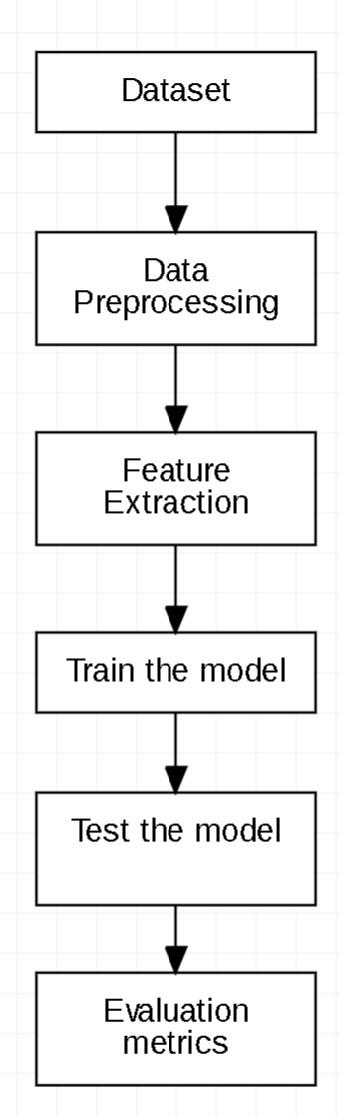
\includegraphics[width=2in]{images/ww1.jpg} 
	\caption{Working mechanism of Network Intrusion Detection System} %figure name
	\label{Working mechanism of Network Intrusion Detection System} % for referencing
\end{center}
\end{figure}
\newpage
\subsection{Data set}
\vspace{-18pt}
InSDN is a comprehensive Software-Defined Network (SDN) dataset for Intrusion detection system evaluation. The new dataset includes the benign and various attack categories  that can occur in different elements of the SDN standard. InSDN considers different attack, including DoS, DDoS, brute force attack, web applications, exploitation, probe, and botnet. Furthermore, the normal traffic in the generated data covers  various  popular  application services such as HTTPS, HTTP, SSL, DNS, Email, FTP, SSH, etc. The dataset was generated by using four virtual machines (VMs). The first virtual machine is a Kali Linux one and represents the attacker server. The secondary machine is a Ubuntu 16.4 one, and acts on the ONOS controller. Third is an Ubuntu 16.4 machine to serve for the Mininet and OVS switch. The forth virtual machine is a Linux one based on metasploitable 2 to provide vulnerable services for demonstrating common vulnerabilities.\cite{article}
\begin{figure}[h] % tbh means top, bottom or here (priority: left to right)
\begin{center}
	%
\includegraphics[width = 3in]{images/logo.png}
	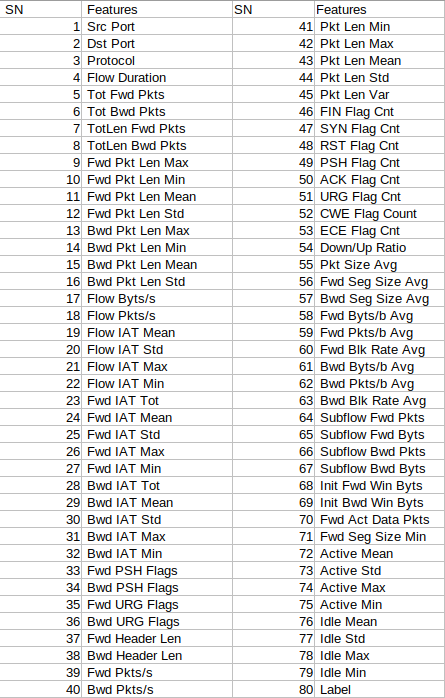
\includegraphics[width=3in]{images/ds2.png} 
	\caption{Features of InSDN dataset} %figure name
	\label{} % for referencing
\end{center}
\end{figure}
\subsection{Data Preprocessing}
\vspace{-18pt}
We used the InSDN dataset. Because the input should be a numeric matrix, we must convert some non-numeric features, into numeric form using label encoding. For the efficient training of neural networks, input data should be transformed by performing some pre-processing known as data normalization. It is used where inputs are widely divergent. Without such a process, networks would take a long time to train. Different schemes can be used to normalise the input data before it is fed to the input layer of neural network. We have used Z-score normalization to normalize the attributes of our dataset. Z-score normalization refers to the process of normalizing every value in a dataset such that the mean of all of the values is 0 and the standard deviation is 1. Mathematically,
\begin{equation}
New value = \frac{x- \mu}{\lambda}
\end{equation}
where $x: $ Original value,\\ $\mu: $ Mean of data,\\ $\lambda: $ Standard deviation of data.
\subsection{Feature Extraction}
\vspace{-18pt}
Principal component analysis, or PCA, is a statistical procedure that allows you to summarize the information content in large data tables by means of a smaller set of  “summary indices” that can be more easily visualized and analyzed.
Algorithm for PCA is given as:
\begin{enumerate}[label=\roman*.]
\item $\mu = \frac{1}{p} \sum_{k=1}^{p} x_{k},$ where, $x_{k}$ is a pattern, $p =$ number of patterns, $x$ is the feature matrix.
\item Find the covariance matrix\\
$ C = \frac{1}{p} \sum_{k=1}^{p}(x_{k} - \mu)(x_{k} - \mu)^{T}$ where T represents matrix transposition.
\item Compute Eigen values $\lambda_{i}$ and Eigen vectors $v_{i}$ of covariance matrix\\
$Cv_{i} = \lambda_{i}v_{i}$\quad \quad \quad \quad$ (i = 1,2,3...q), q =$ number of features
\item Estimating high-valued Eigen vectors
\begin{enumerate}
\item Arrange all the Eigen values $(\lambda_{i})$ in descending order.
\item Choose a threshold value, $\theta$
\item Number of high-valued $\lambda_{i}$ can be chosen so as to satisfy the relationship\\
$(\sum_{i=1}^{s}\lambda_{i})(\sum_{i=1}^{q}\lambda_{i})^{-1} \geq \theta,$ where $s = $ number of high valued $\lambda_{i}$ chosen 
\item Select Eigen vectors corresponding to selected high valued $\lambda_{i}$
\end{enumerate}
\item Extract low dimensional feature vectors (principal components) from raw feature matrix.\\
$P = V^{T}x$, where $V$ is the matrix of principal components and $x$ is the feature matrix.
\end{enumerate}
\subsection{Train and test the model}
\vspace{-18pt}
The model used in this project for NIDS is: Long Shortterm Memory (LSTM).
\par 
\subsubsection{Long Short term Memory (LSTM)}
\vspace{-18pt}
LSTM is a popular deep learning technique in RNN for time series prediction. While standard RNNs outperform traditional networks in preserving information, they are not very effective in learning long term dependencies due to the vanishing gradient problem. An LSTM is well-suited to classify and/or predict time-series data. There are several architectures of LSTM units. A common architecture is composed of a memory cell, an input gate, an output gate and a forget gate. The mathematical formulation of the LSTM cell is given below:
\begin{eqnarray}
f_t = \sigma(x_tW_f + H_{t-1}U_f)\\
o_t = \sigma(x_tW_o + H_{t-1}U_o)\\
S_t = \sigma(S_{t-1} *f_t + i_t * H^{'}_t)\\
i_t = \sigma(x_tW_i + H_{t-1}U_i)\\
H^{'}_t = tanh(x_tW_g + H_{t-1}U_g)\\
H_t = tanh(S_t)*o_t
\end{eqnarray}
\begin{figure}[tbh] % tbh means top, bottom or here (priority: left to right)
\begin{center}
	%
\includegraphics[width = 3in]{images/logo.png}
	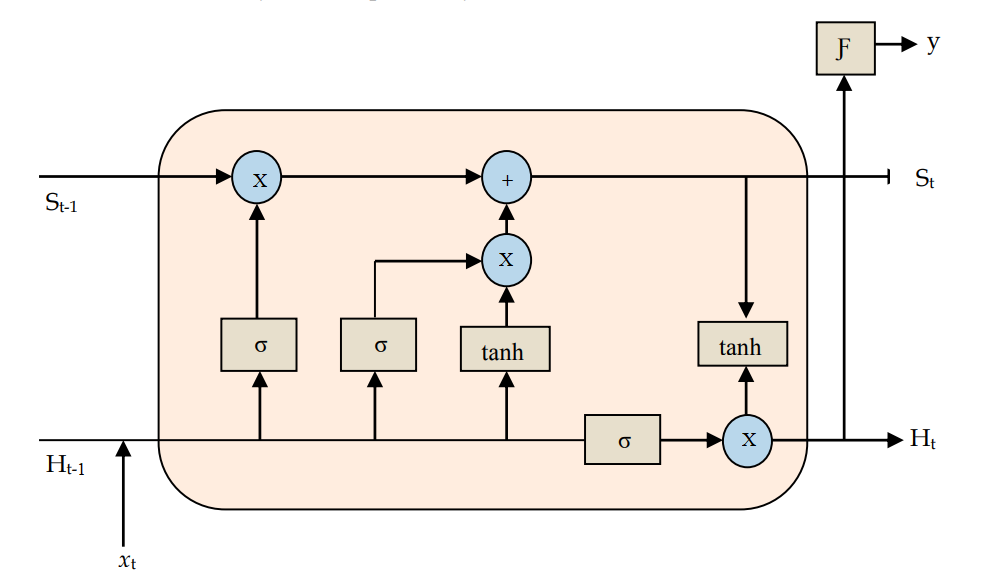
\includegraphics[width=6in]{images/l1.png} 
	\caption{LSTM} %figure name
	\label{LSTM} % for referencing
\end{center}
\end{figure}
\newpage
\subsection{Evaluation Metrics}
\vspace{-18pt}
The most important performance indicator (Accuracy, AC) of intrusion detection is used to measure the performance of the model. In addition to the accuracy, we introduce the detection rate and false positive rate. The True Positive (TP) is equivalent to those correctly rejected, and it denotes the number of anomaly records that are identified as anomaly. The False Positive (FP) is the equivalent of incorrectly rejected, and it denotes the number of normal records that are identified as anomaly. The True Negative (TN) is equivalent to those correctly admitted, and it denotes the number of normal records that are identified as normal. The False Negative (FN) is equivalent to those incorrectly admitted, and it denotes the number of anomaly records that are identified as normal.
\begin{figure}[tbh] % tbh means top, bottom or here (priority: left to right)
\begin{center}
	%
\includegraphics[width = 3in]{images/logo.png}
	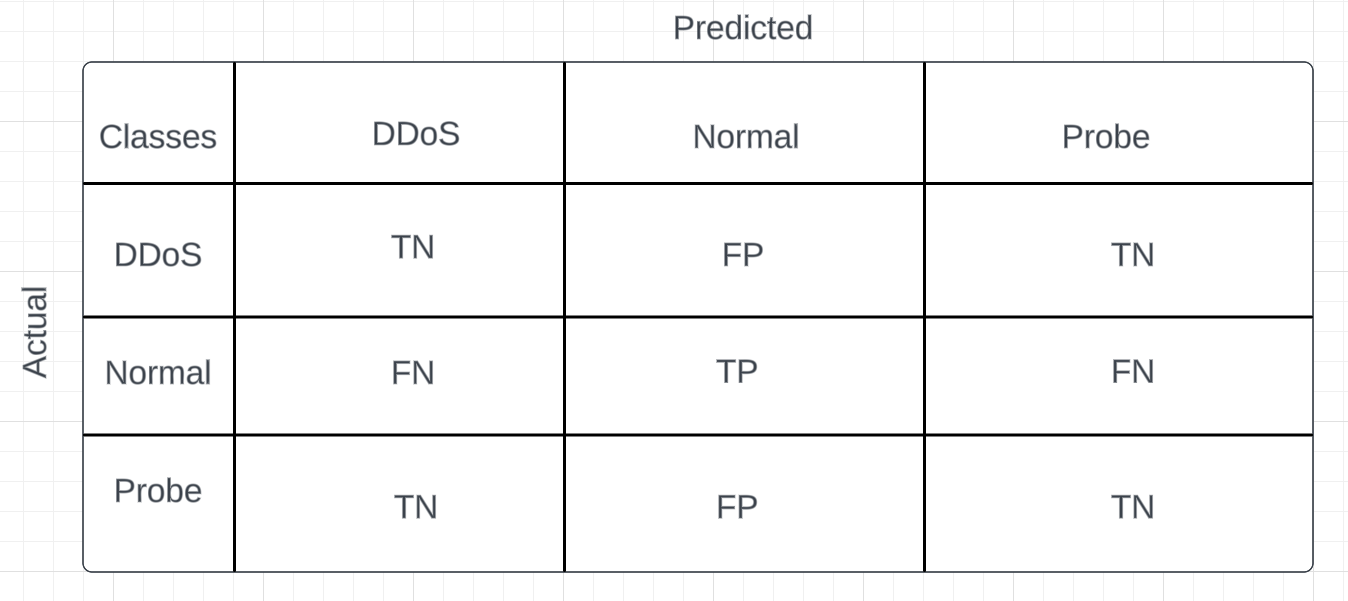
\includegraphics[width=6in]{images/confMat.png} 
	\caption{Confusion Matrix} %figure name
	\label{Confusion Matrix} % for referencing
\end{center}
\end{figure}
\begin{equation}
Accuracy = \frac{TP + TN}{TP + TN + FP + FN}
\end{equation} 
Precision is the number of actual attacks as a proportion of the number classified as attacks.
\begin{equation}
Precision = \frac{TP}{TP + FP} 
\end{equation}
True Positive Rate shows the percentage of the number of records identified correctly over the total number of anomaly records.
\begin{equation}
True Positive Rate = \frac{TP}{FN + TP}
\end{equation}
False Positive Rate is the percentage of the number of records rejected incorrectly is divided by the total number of normal records.
\begin{equation}
False Positive Rate = \frac{FP}{FP + TN}
\end{equation}
\section{System Diagram}
\vspace{-18pt}
\subsection{Use case diagram}
\begin{figure}[h]
\begin{center}
	%
\includegraphics[width = 3in]{images/logo.png}
	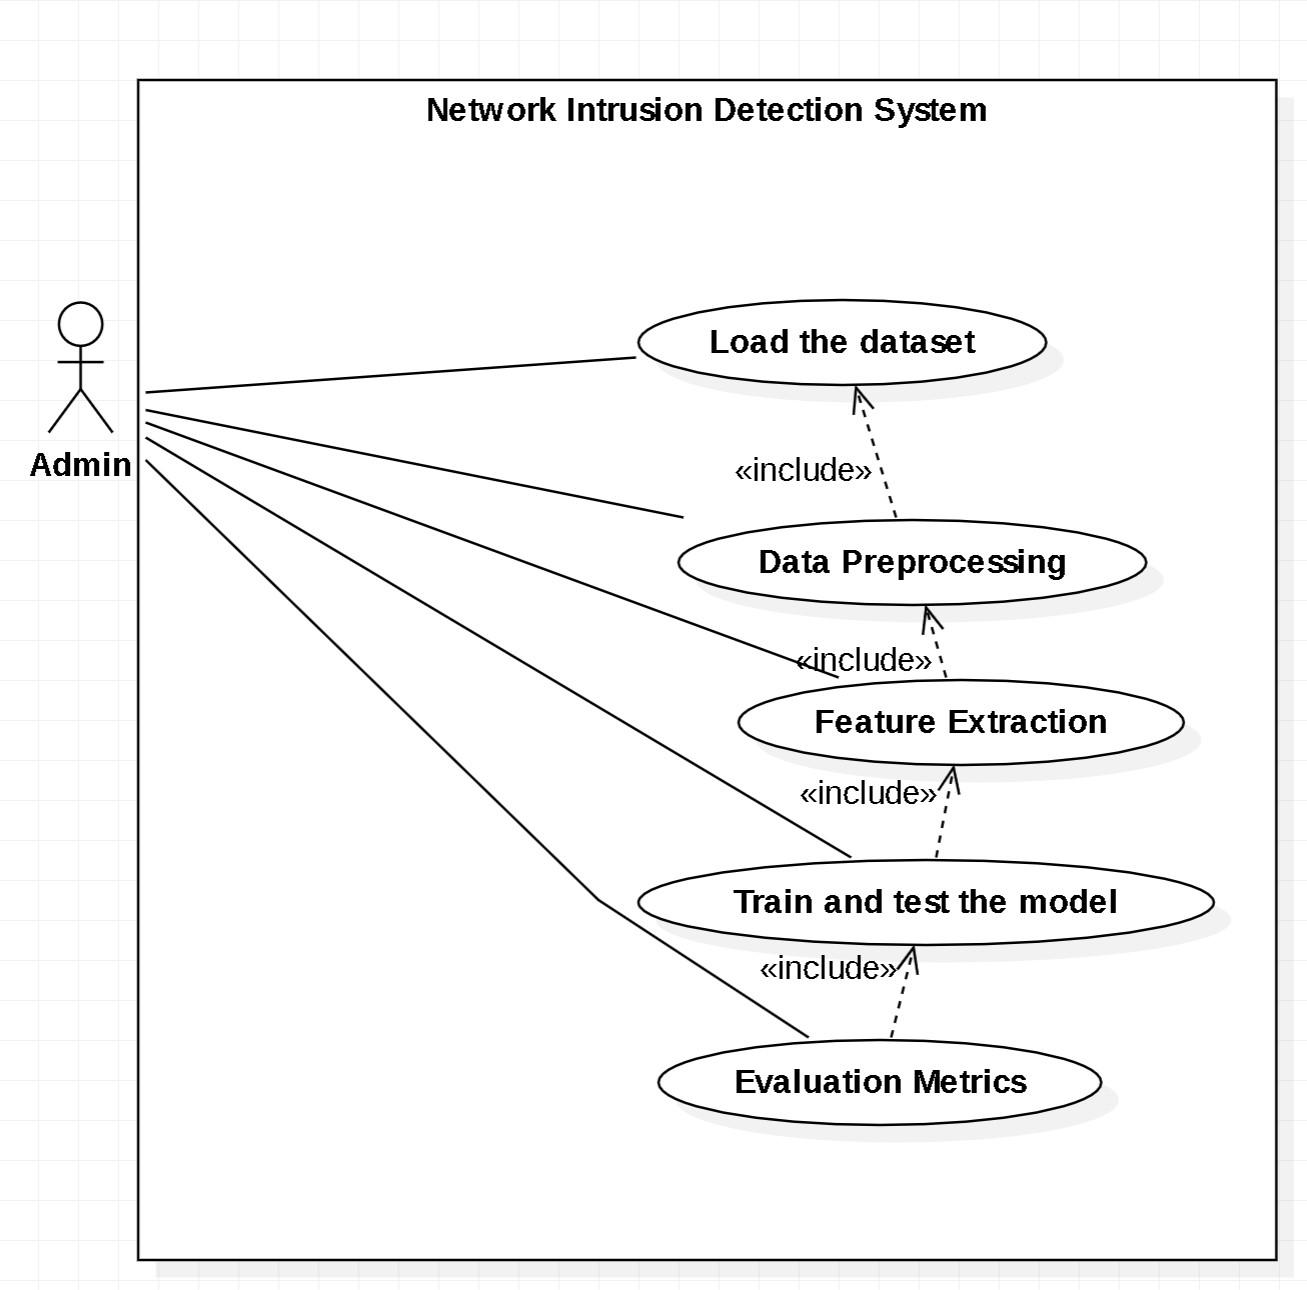
\includegraphics[width=5in]{images/use.jpg} 
	\caption{Use case Diagram of Network Intrusion Detection System} %figure name
	\label{Use case Diagram of Network Intrusion Detection System} % for referencing
\end{center}
\end{figure}
\newpage
\subsection{Software Development Model}
\vspace{-18pt}
 \begin{figure}[tbh] % tbh means top, bottom or here (priority: left to right)
\begin{center}
	%
\includegraphics[width = 3in]{images/logo.png}
	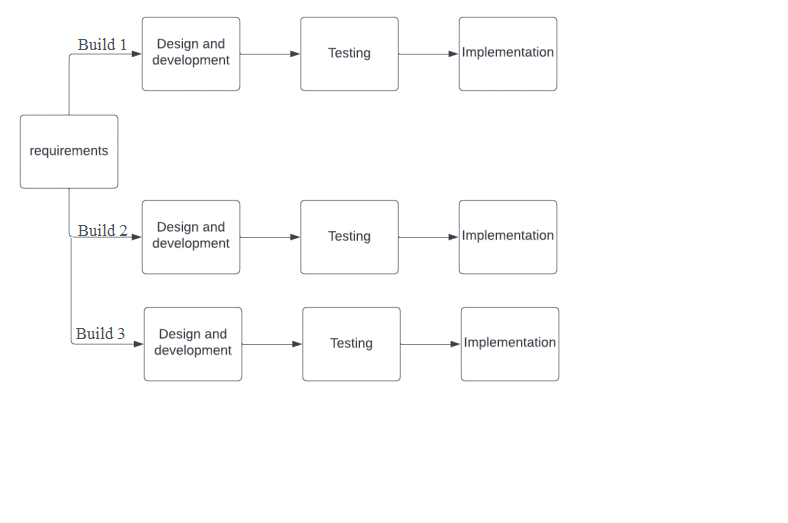
\includegraphics[width=6in]{images/sdlc1.png} 
	\caption{Incremental Model} %figure name
	\label{Incremental Model} % for referencing
\end{center}
\end{figure}
Incremental model is a method of software engineering that combines the elements of waterfall model in iterative manner. It involves both development and maintenance. In this model requirements are broken down into multiple modules. Incremental development is done in steps from analysis design, implementation, testing/verification, maintenance. Each iteration passes through the requirements, design, coding and testing phases. The first increment is often a core product where the necessary requirements are addressed, and the extra features are added in the next increments. The core product is delivered to the client. Once the core product is analyzed by the client, there is plan development for the next increment.
\chapter{Results and Discussion}
\vspace{-18pt}
\section{Result}
\vspace{-18pt}
We have completed the development of the project along with obtaining the desirable output. We divided the original dataset into train and test set with 80/20 split. We then trained the LSTM model for the train set and checked the classification report and confusion matrix for both the test set and the validation set that we created.

\begin{figure}[tbh] % tbh means top, bottom or here (priority: left to right)
	\begin{center}
		%
\includegraphics[width = 3in]{images/logo.png}
		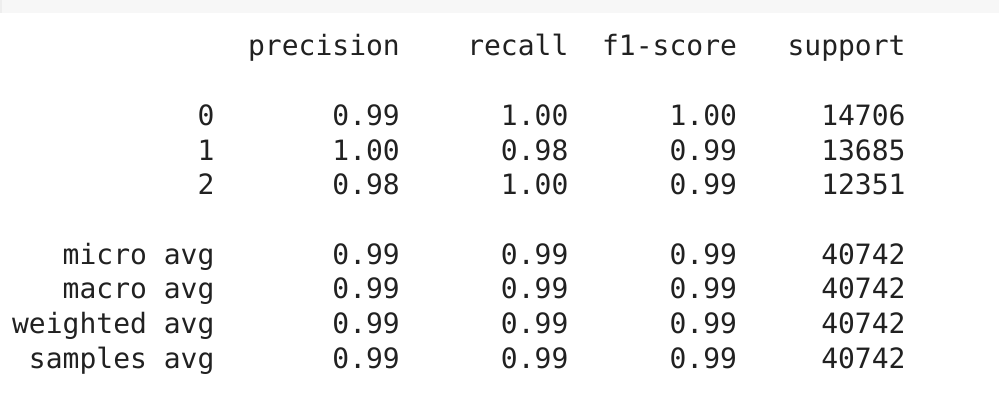
\includegraphics[width=3in]{images/cReportTest.png} 
		\caption{Classification Report for Test dataset} %figure name
		\label{Classification Report for Test dataset} 
	\end{center}
\end{figure}
\begin{figure}[tbh] % tbh means top, bottom or here (priority: left to right)
	\begin{center}
		%
\includegraphics[width = 3in]{images/logo.png}
		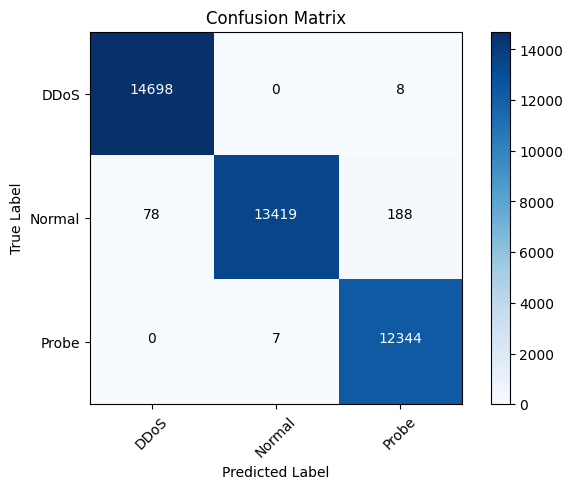
\includegraphics[width=4in]{images/confMatTest.png} 
		\caption{Confusion Matrix for Test dataset} %figure name
		\label{Confusion Matrix for Test dataset} 
	\end{center}
\end{figure}
\begin{figure}[tbh] % tbh means top, bottom or here (priority: left to right)
	\begin{center}
		%
\includegraphics[width = 3in]{images/logo.png}
		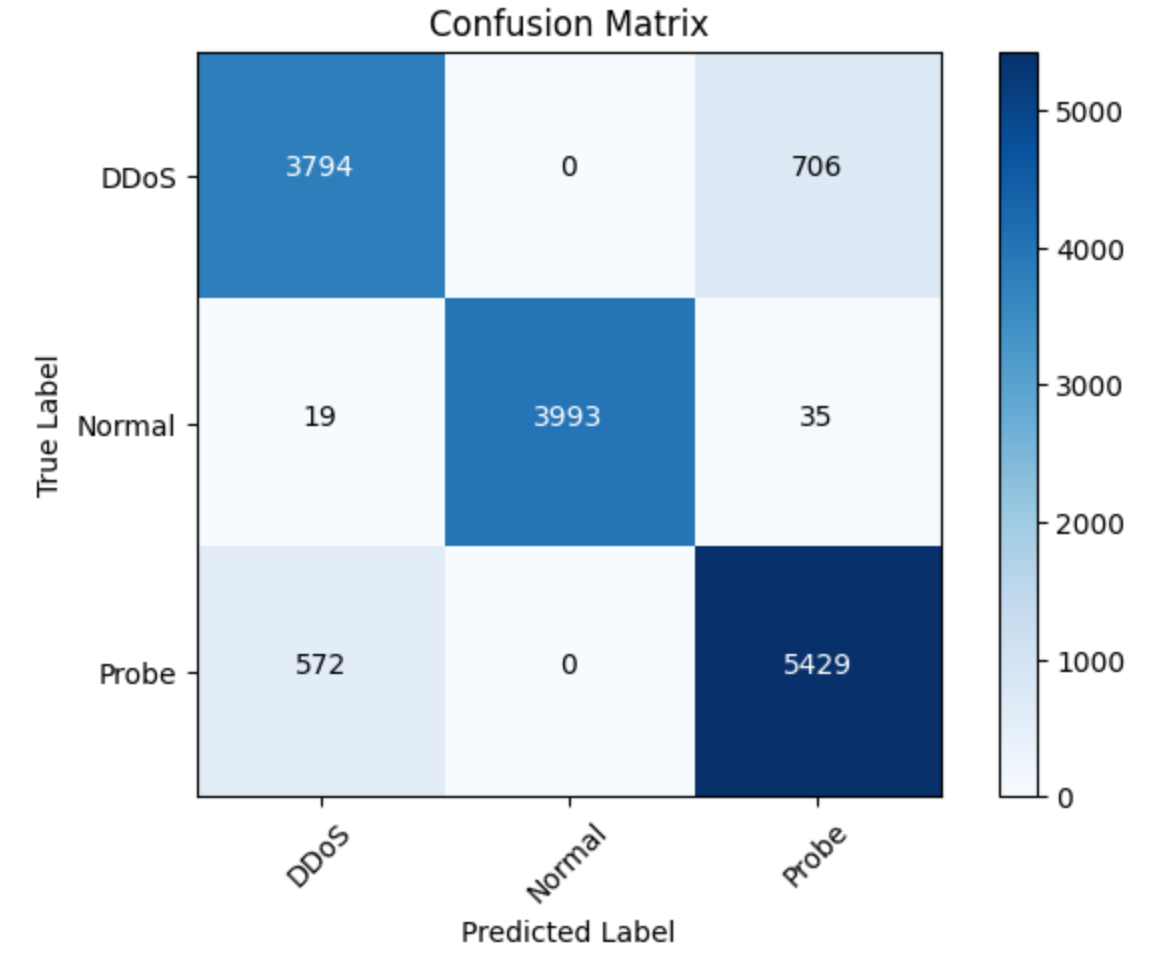
\includegraphics[width=4in]{images/confMatVal.png} 
		\caption{Confusion Matrix for Validation dataset} %figure name
		\label{Confusion Matrix for Validation dataset} 
	\end{center}
\end{figure}
\begin{figure}[tbh] % tbh means top, bottom or here (priority: left to right)
	\begin{center}
		%
\includegraphics[width = 3in]{images/logo.png}
		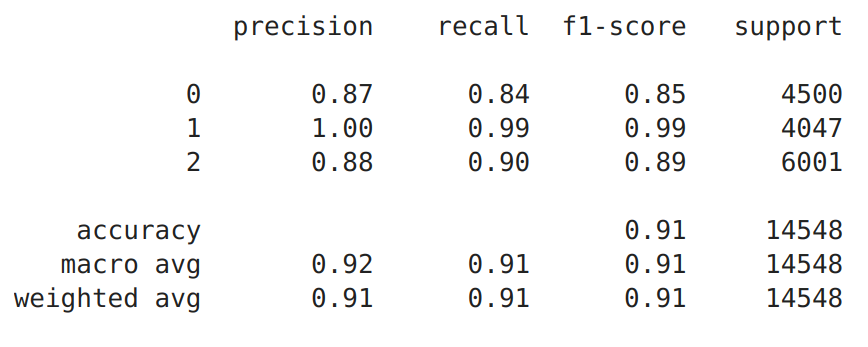
\includegraphics[width=3in]{images/cReportVal.png} 
		\caption{Classification Report for Validation dataset} %figure name
		\label{Classification Report for Validation dataset} 
	\end{center}
\end{figure}
\newpage
In the above figures, 0 denotes DDoS class, 1 denotes Normal class and Probe class is denoted by 2. As we can see, the model achieved 91\% accuracy for prediction of the labels in the validation set.
\section{Discussion}
\vspace{-18pt}
bla bla bla
\section{Limitations}
\begin{enumerate}
	\item hmmm
	\item mmmm
\end{enumerate}
\chapter{Conclusion and Future Enhancements}
\vspace{-18pt}
\section{Conclusion}
\vspace{-18pt}
blablablabla
\section{Future Enhancements}
\begin{enumerate}
	\item bla bla
	\item bla bla
\end{enumerate}
%Reference
\renewcommand\bibname{References} % Change heading to References
\bibliographystyle{IEEEtran} % to use IEEE Format for referencing
\addcontentsline{toc}{chapter}{References} % to add references in TOC
\bibliography{library} % specify the .bib file containing reference information 
\end{document}
